\subsection{Preliminaries}
We have already defined the \ssc problem, but for our analysis, we need some more definitions. In particular, we first define a Gomory-Hu Steiner tree and its approximation version.

\BD[Gomory-Hu Steiner tree]
Given a graph $G=(V,E)$ and a set of terminals $U\s V$, the Gomory-Hu Steiner tree is a weighted tree $T$ on the vertices $U$, together with a function $f:V\to U$, such that
 \BI
 \im For all $s,t\in U$, consider the minimum-weight edge $(u,v)$ on the unique $s-t$ path in $T$. Let $U'$ be the vertices of the connected component of $T-(u,v)$ containing $s$.
Then, the set $f\inv(U')\s V$ is an $(s,t)$-mincut, and its value is $w_T(u,v)$.
 \EI
\ED

\BD[Approximate Gomory-Hu Steiner tree]
Given a graph $G=(V,E)$ and a set of terminals $U\s V$, the $(1+\e)$-approximate Gomory-Hu Steiner tree is a weighted tree $T$ on the vertices $U$, together with a function $f:V\to U$, such that
 \BI
 \im For all $s,t\in U$, consider the minimum-weight edge $(u,v)$ on the unique $s-t$ path in $T$. Let $U'$ be the vertices of the connected component of $T-(u,v)$ containing $s$.
Then, the set $f\inv(U')\s V$ is a $(1+\e)$-approximate $(s,t)$-mincut, and its value is $w_T(u,v)$.
 \EI
\ED

It would also be useful in our analysis to use the notion of a {\em minimal} Gomory-Hu tree. We define this next.

\BD[Rooted minimal Gomory-Hu Steiner tree]\label{defn:minimalGH}
Given a graph $G=(V,E)$ and a set of terminals $U\s V$, a rooted minimal Gomory-Hu Steiner tree is a Gomory-Hu Steiner tree on $U$, rooted at some vertex $r\in U$, with the following additional property:
 \BI
% MORE GENERAL BUT HARDER TO PROVE, SO WE SKIPPED -> \im[$(*)$] For all $s,t\in U$ where $s$ is a descendant of $t$ in the rooted tree $T$, consider the minimum-weight edge $(u,v)$ on the unique $s-t$ path in $T$; if there are multiple minimum weight edges, let $(u, v)$ denote the one that is {\em closest to $s$}. Let $U'$ be the vertices of the connected component of $T-(u,v)$ containing $s$.
 \im[$(*)$] For all $t\in U\sm\{r\}$, consider the minimum-weight edge $(u,v)$ on the unique $r-t$ path in $T$; if there are multiple minimum weight edges, let $(u, v)$ denote the one that is {\em closest to $t$}. Let $U'$ be the vertices of the connected component of $T-(u,v)$ containing $r$.
Then, $\pt_Gf\inv(U')\s V$ is a \emph{minimal} $(r,t)$-mincut, and its value is $w_T(u,v)$.
 \EI
\ED

The following theorem, proved in the appendix, establishes the existence of a rooted minimal Gomory-Hu Steiner tree rooted at any given vertex.

\begin{restatable}{theorem}{Rooted}\thml{rooted}
For any graph $G=(V,E)$, terminals $U\s V$, and root $r\in U$, there exists a rooted minimal Gomory-Hu Steiner tree rooted at $r$.
\end{restatable}


\subsection{Algorithms for the \ct and \ssc Problems}

As described earlier, the main tool in our \ssc algorithm is an algorithm for the Cut Threshold (\ct) problem. We first describe a single step of the \ref{thr} algorithm (we call this \ref{step}):

%\alert{This section starts abruptly. Let us add a text description of what we are going to in this section, and a short outline of the algorithm.} 

\begin{algorithm}
\mylabel{step}{\textsc{CutThresholdStep}}\caption{\ref{step}$(G=(V,E),s,U,W)$} 
\begin{algorithmic}[1]
\State Initialize $R^0\gets U$ and $D\gets\emptyset$
\For{$i$ from $0$ to $\lf\lg|U|\rf$}
 \State Compute minimum isolating cuts $\{S^i_v:v\in R^i\}$ on inputs $G$ and $R^i$ \linel{Sv}
 \State Let $D^i$ be the union of $S^i_v\cap U$ over all $v\in R^i\sm \{s\}$ satisfying $w(\pt S^i_v)\le W$
 \State $R^{i+1}\gets$ subsample of $R^i$ where each vertex in $R^i\sm \{s\}$ is sampled independently with probability $1/2$, and $s$ is sampled with probability $1$
\EndFor
%\State $D\gets D^0\cup D^1\cup \cds\cup D^{\lf\lg|U|\rf}$
\State\Return $D^0\cup D^1\cup \cds\cup D^{\lf\lg|U|\rf}$
\end{algorithmic}
\end{algorithm}

Let $D=D^0\cup D^1\cup \cds\cup D^{\lf\lg|U|\rf}$ be the union of the sets output by the algorithm. We first introduce the following lemma which will work for all $D^*$ that is downward-closed in the tree $T$ rooted at $s$. We will later set $D^*$ as all vertices $v\in U\sm \{s\}$ for which the $(s,v)$-mincut has weight at most $W$. 

\BL\leml{step}
For any downward-closed set $D^*$
$D\s D^*$ and $\E[|D|] = \Om(|D^*|/\log|U|)$. 
\EL
\BP
We first prove that $D\s D^*$. Each vertex $u\in D$ belongs to some $S^i_v$ satisfying $w(\pt S^i_v)\le W$. %and $S^i_v\cap U=\{v\}$ for some $v\in U\sm s$. 
In particular, $\pt S^i_v$ is an $(s,u)$-cut with weight at most $ W$. It follows that the $(s,u)$-mincut also has weight at most $ W$, and therefore, $u\in D$.

It remains to prove that $\E[|D|]\ge\Om(|D^*|/\log|U|)$. Consider a rooted minimal Steiner Gomory-Hu tree $T$ of $G$ on terminals $U$ rooted at $s$, which exists by \thm{rooted}. By definition of the Steiner Gomory-Hu tree, a vertex $v\in U$ is in $D^*$ iff its path to the root $s$ in $T$ has at least one edge of weight at most $ W$. For each vertex $v\in U\sm \{s\}$, let $r(v)$ be defined as the child vertex of the lowest weight edge on the path from $v$ to $s$ in $T$. If there are multiple lowest weight edges, choose the one with the maximum depth. %\alert{The lowest weight edge is unique because there is only one $(v,s)$-mincut.}

%\alert{DP: 1. Need to define rooted minimal Steiner Gomory-Hu tree which is used in the para above. 3. Should we talk about breaking ties among multiple lowest weight edges or add a perturbation at the outset and claim that mincuts are unique? This last fact needs a proof since there could be exponential number of $s-t$ mincuts, so just adding an inverse polynomial perturabtion does not immediately imply uniqueness. But, perhaps use the (classic) isolation lemma?} \textcolor{blue}{I had assumed all $s-t$ mincuts unique in a previous write-up. I do think the new version is better since we also obtain better bounds for unweighted graphs which we can't use isolation lemma for. But maybe a note to the reader that assuming all min-cuts are unique could help with a first reading}

For each vertex $v\in D^*$, consider the subtree rooted at $v$, define $U_v$ to be the vertices in the subtree, and define $n_v$ as the number of vertices in the subtree. We say that a vertex $v\in D^*$ is \emph{active} if $v\in R^i$ for $i=\lf\lg n_{r(v)}\rf$. In addition, if $U_{r(v)}\cap R^i=\{v\}$, then we say that $v$ \emph{hits} all of the vertices in $U_{r(v)}$ (including itself); see Figure~\ref{fig:hits}. In particular, in order for $v$ to hit any other vertex, it must be active. For completeness, we say that any vertex in $U\sm D^*$ is not active and does not hit any vertex.

%\alert{The above definitions are fine, but would be easier to read with (a) some intuition behind when you say that a vertex is active and process of hitting other vertices, and (b) a figure illustrating the notation.} 

%\textcolor{blue}{Jason: added a figure.}

\begin{figure}\centering
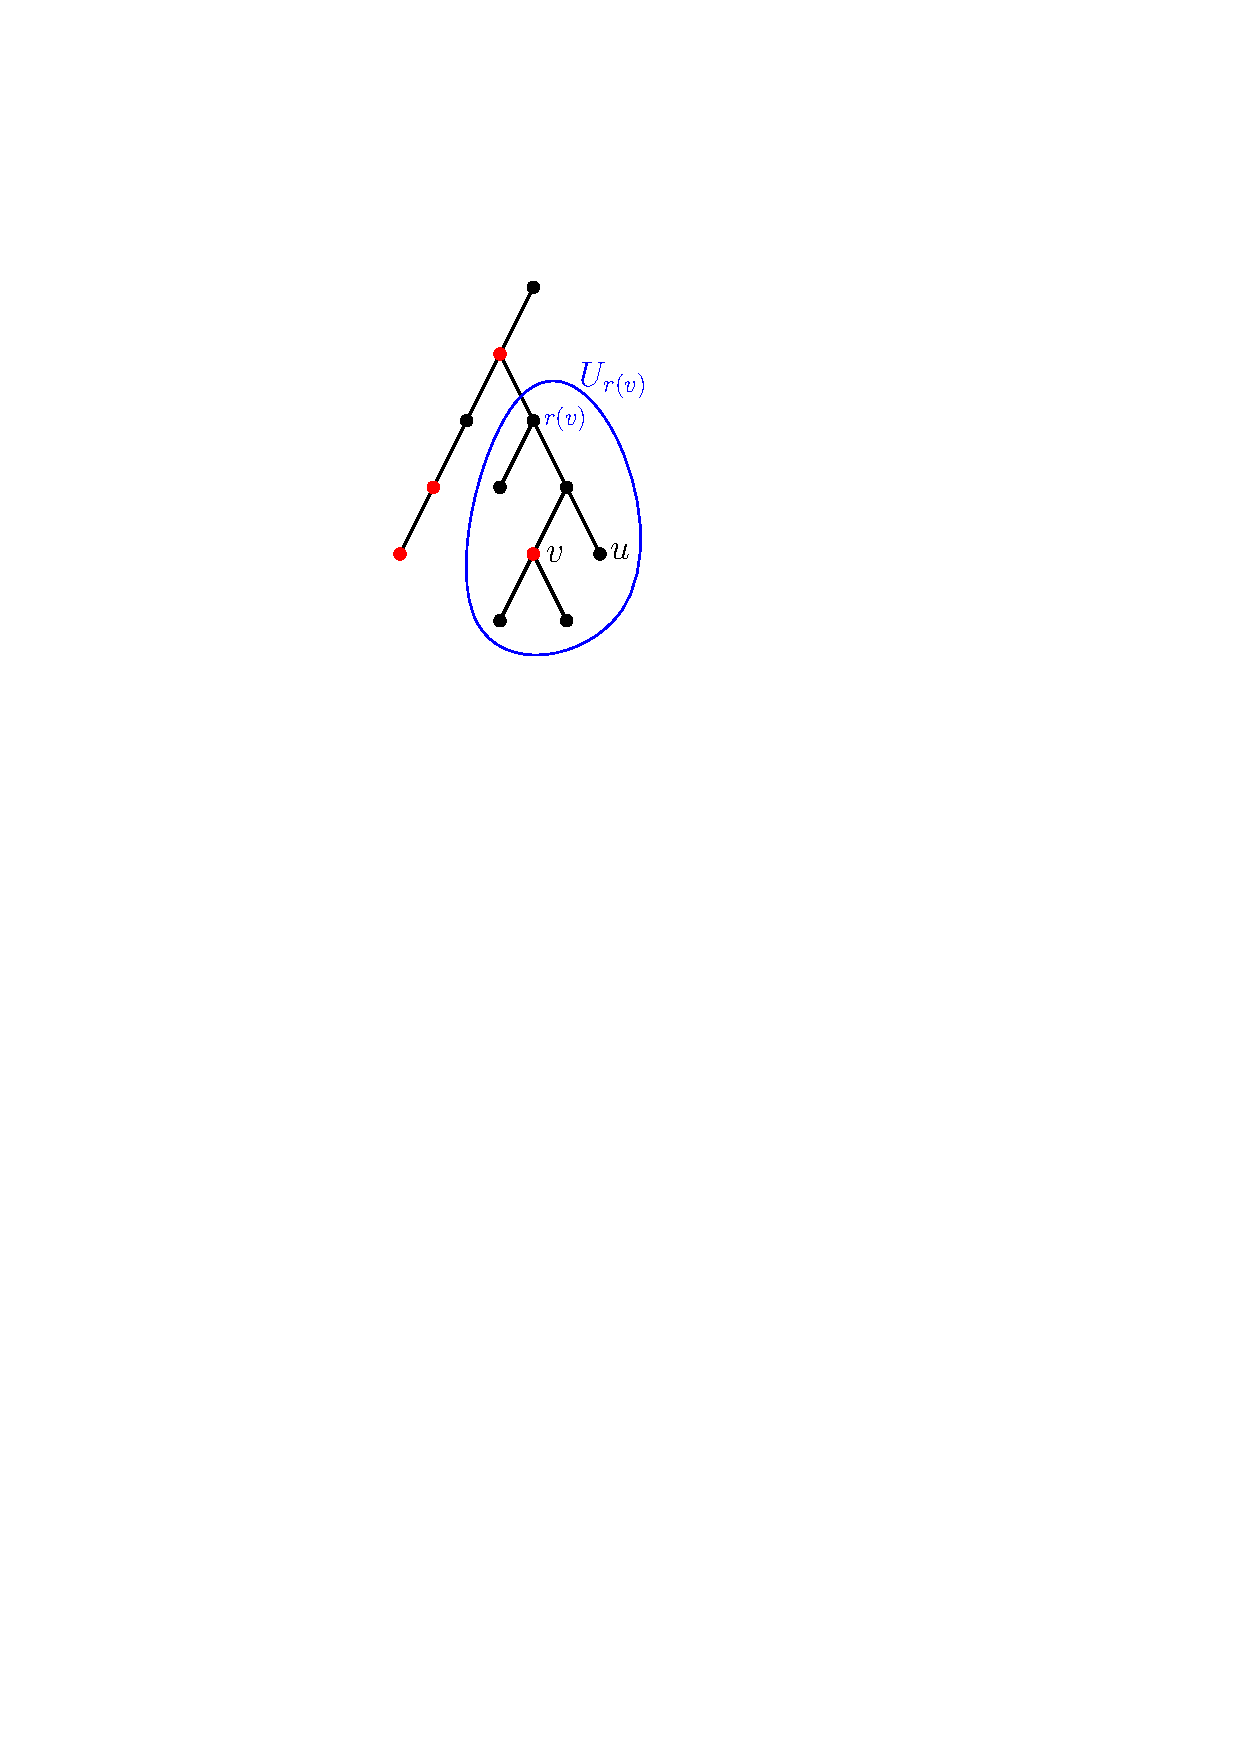
\includegraphics[scale=1]{hits.pdf}
\caption{Let $i=\lf\lg n_{r(v)}\rf=\lf\lg 7\rf=2$, and let the red vertices be those sampled in $R^2$. Vertex $v$ is active and hits $u$ because $v$ is the only vertex in $U_{r(v)}$ that is red.}\label{fig:hits}
\end{figure}

To prove that $\E[|D|] \ge \Om(|D^*|/\log|U|)$, we will show that
 \BE
 \im[(a)] each vertex $u$ that is hit is in $D$, 
 \im[(b)] the total number of pairs $(u,v)$ for which $v\in D^*$ hits $u$ is at least $c |D^*|$ in expectation for some small enough constant $c>0$, and
 \im[(c)] with probability at least $1-\f c{2|U|^2}$ (for the constant $c>0$ in~(b)), each vertex $u$ is hit by at most $O(\log|U|)$ vertices $v\in D^*$. %\alert{DP: There's some play on constants here between the constant hidden in $O(.)$ and the constant in the denominator? Should we make this more explicit?}
 \EE

For (a), consider the path from $u$ to the root $s$ in $T$, and take any vertex $v\in D^*$ on the path that is active (possibly $u$ itself). Such a vertex must exist since $u$ is hit by some vertex. By definition, for $i=\lf\lg n_{r(v)}\rf$, we have $U_{r(v)}\cap R^i=\{v\}$, so $\pt U_{r(v)}$ is a $(v,R^i\sm \{v\})$-cut.  By the definition of $r(v)$, we have that $\pt U_{r(v)}$ is a $(v,s)$-mincut. On the other hand, we have that $\pt f\inv(S^i_v)$ is a $(v,R^i\sm v)$-mincut, so in particular, it is a $(v,s)$-cut. It follows that $\pt f\inv(U_{r(v)})$ and $\pt f\inv(S^i_v)$ are both $(v,s)$-mincuts and $(v,R^i\sm v)$-mincuts. Since $T$ is a minimal Gomory-Hu Steiner tree, we must have $f\inv(U_{r(v)}) \s S^i_v$. Since $u\in U_{r(v)}\s f\inv(U_{r(v)})\s S^i_v$, it is added to $D$ on \line{Sv}. 

For (b), for $i=\lf\lg n_{r(v)}\rf$, we have $v\in R^i$ with probability exactly $1/2^i = \Th(1/n_{r(v)})$, and with probability $\Om(1)$, no other vertex in $U_{r(v)}$ joins $R^i$. Therefore, $v$ is active with probability $\Om(1/n_{r(v)})$. Conditioned on $v$ being active, it hits exactly $n_{r(v)}$ many vertices. It follows that $v$ hits $\Om(1)$ vertices in expectation.

For (c), the number of vertices $v$ that hit vertex $u$ is at most the number of active vertices $v$ for which $r(v)$ is on the path from $u$ to $s$ in $T$. Label these vertices $u=v_1,v_2,\lds,v_\el=s$, ordered by increasing distance from $u$ to $r(v_i)$ in $T$. Each vertex $v_j\in D^*$ is active with probability $\Th(1/n_{r(v_j)})$, which is at most $\Th(1/j)$ since $v_1,\lds,v_j \in U_{r(v_j)}$. Each vertex $v_j\notin D^*$ is never active. Therefore, the expected number of active vertices on the path from $u$ to $s$ is at most $\sum_{j=1}^\el\Th(1/j)=\Th(\ln\el)\le \Th(\ln|U|)$. A standard Chernoff bound shows that with probability at least $1-\f c{2|U|^3}$ for any constant $c>0$, the number of active vertices on the path is indeed $O(\ln|U|)$, where the $O(\cd)$ hides the dependency on $c$. Taking a union bound over all $u\in U$, the probability that this is true for all vertices is at least $1-\f c{2|U|^2}$.

Finally, we show why properties (a) to (c) imply $\E[|D|] \ge \Om(|D^*|/\log|U|)$. In the event that property~(c) fails, the total number of pairs $(u,v)$ for which $v$ hits $u$ can be trivially upper bounded by $|U|^2$. Since this occurs with probability at most $\f c{2|U|^2}$, the total contribution to the expectation $c|D^*|$ in property~(b) is at most $c/2$. Therefore, the contribution to the expectation in the event that property~(c) succeeds is at least $c|D^*|-c/2\ge (c/2)|D^*|$. In this case, since each vertex is hit at most $O(\log|U|)$ times, there are at least $\Om(|D^*|/\log|U|)$ vertices hit in expectation.
\EP

%The following corollary will be useful in the next section:
%\BC\corl{Dmax}
%Let $D_{\max}$ be the largest set $\bigcup_{v\in R^i} (S^i_v\cap U)$ over all iterations $i$, and let $i_{\max}$ be the corresponding iteration. Then, $\E[|D_{\max}|] \ge \Om(|D^*|/\log^2|U|)$.
%\EC
%\BP
%There are $\lf\lg{U}\rf+1$ iterations in which we add to $D$, so $|D_{\max}|\ge |D|/(\lf\lg|U|\rf+1)$.
%Combining this with $\E[|D|]\ge\Om(|D^*|/\log|U|)$ from \lem{step} proves the claim. 
%\EP

We now use iterate Algorithm~\ref{step} to obtain the \ref{thr} algorithm:

\begin{algorithm}
\mylabel{thr}{\textsc{CutThreshold}}\caption{\ref{thr}$(G=(V,E),s, W)$}
\begin{algorithmic}[1]
\State Initialize $U\gets V$ and $D_{\textup{total}}\gets\emptyset$
\For{$O(\log^2n)$ iterations}
 \State Let $D$ be the union of the sets output by $\ref{step}(G,s,U, W)$
 \State Update $D_{\textup{total}}\gets D_{\textup{total}}\cup D$ and $U\gets U\sm D$
\EndFor
\State\Return $D_{\textup{total}}$
\end{algorithmic}
\end{algorithm}


\BC\corl{threshold}
W.h.p., the output $D_{\textup{total}}$ of \ref{thr} is exactly all vertices $v\in U\sm \{s\}$ for which the $(s,v)$-mincut has weight at most $ W$. 
\EC
\BP
%Let $D^*$ be the targeted output.
By \lem{step}, $|U\cap D^*|$ decreases by $\Om(|D^*|/\log n)$ in expectation. After $O(\log^2n)$ iterations, we have $\E[|U\cap D^*|] \le 1/\poly(n)$, so w.h.p., $U\cap D^*=\emptyset$. Each vertex in $D^*$ that is removed from $U$ is added to $D_{\textup{total}}$, and no vertices in $U\sm D^*$ are added to $D_{\textup{total}}$, so w.h.p., the algorithm returns the correct set $D^*$.
\EP
In other words, \ref{thr} is an algorithm that fulfills \thm{thr}, restated below.
\Thr*

Finally, we use the \ref{thr} algorithm to design our \ssc algorithm:

\begin{algorithm}
\caption{\textsc{ApproxSSMC}$(G=(V,E),s,\e)$}
\begin{algorithmic}[1]
 \State Initialize bounds: $ w_{\min} \gets$ minimum weight of an edge in $G$, and $ w_{\max}\gets$ maximum weight of an edge %\Comment{Every $(s,v)$-mincut has weight in $[ w_{\min}, w_{\max}]$}
 \For{all integers $j\ge0$ s.t.\ $(1+\e)^j w_{\min} \in [ w_{\min},(1+\e) n w_{\max}]$}
 \State $ W_j\gets (1+\e)^j w_{\min}$
 \State $D_j\gets \ref{thr}(G,s, W)$
\EndFor
\State For each vertex $v\in V$, take the largest $D_i$ containing $v$, and set $\tilde\la(v)\gets  W_i$
\State\Return $\tilde\la:V\to \R$
\end{algorithmic}
\end{algorithm}

\BL
W.h.p., the output $\tilde\la$ of \textsc{ApproxSSMC} satisfies $\mincut(s,v) \le \tilde\la(v) \le (1+\e)\mincut(s,v)$.
\EL
\BP
For all $v\in V\sm\{s\}$, we have $w_{\min}\le\mincut(s,v)\le w(\pt(\{s\}))\le nw_{\max}$, so there is an integer $j$ with $ W_j\in[\mincut(s,v),(1+\e)\mincut(s,v))$. The lemma follows from \cor{threshold} applied to this $j$.
%Follows from \cor{threshold} and the fact that for all $v\in V$, there is an integer $i$ with $ W_i\in[\mincut(s,v),(1+\e)\mincut(s,v))$. 
\EP

We have therefore proved \thm{ssmc}, restated below.
\SSMC*

